\documentclass[8pt]{article}  % Adjusts the main text font size
\usepackage{paperlighter}
\usepackage[font=small,labelfont=bf]{caption}
% Recommended, but optional, packages for figures and better typesetting:
\usepackage{microtype}
\usepackage{graphicx}
\usepackage{subfigure}
\usepackage{booktabs} % for professional tables
    
    % Attempt to make hyperref and algorithmic work together better:
    \newcommand{\theHalgorithm}{\arabic{algorithm}}
    
    
    % For theorems and such
    \usepackage{amsmath}
    \usepackage{amssymb}
    \usepackage{mathtools}
    \usepackage{amsthm}
    \usepackage{url}
   
    
    % if you use cleveref..
    \usepackage[capitalize,noabbrev]{cleveref}
    
    %%%%%%%%%%%%%%%%%%%%%%%%%%%%%%%%
    % THEOREMS
    %%%%%%%%%%%%%%%%%%%%%%%%%%%%%%%%
    \theoremstyle{plain}
    \newtheorem{theorem}{Theorem}[section]
    \newtheorem{proposition}[theorem]{Proposition}
    \newtheorem{lemma}[theorem]{Lemma}
    \newtheorem{corollary}[theorem]{Corollary}
    \theoremstyle{definition}
    \newtheorem{definition}[theorem]{Definition}
    \newtheorem{assumption}[theorem]{Assumption}
    \theoremstyle{remark}
    \newtheorem{remark}[theorem]{Remark}
    
    % Todonotes is useful during development; simply uncomment the next line
    %    and comment out the line below the next line to turn off comments
    %\usepackage[disable,textsize=tiny]{todonotes}
    \usepackage[textsize=tiny]{todonotes}
    
    
    \begin{document}
    
    \small\lightertitle{Digital Signal Processing - Laboratory Report 3}
    \begin{flushright}
    \textbf{Jan/2024}
    \lighterauthor{Hongyu Rui}
    \end{flushright}




    \section{Laboratory 7}
    \subsection{Task A}
    The estimates of the mean and variance against time of an EEG signal for window lengths of 0.5, 1, 
    and 1.5 seconds are shown below.

    % figure1
   \begin{minipage}{0.5\textwidth}  
    \centering  
    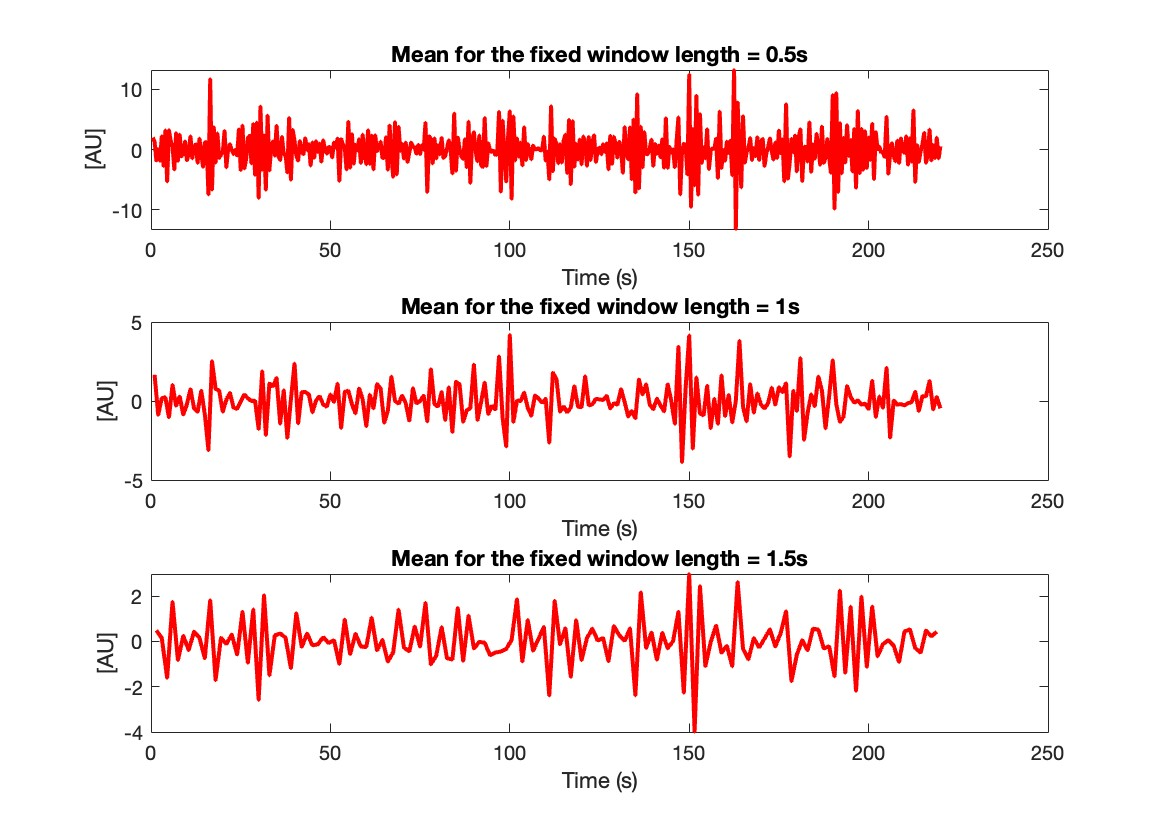
\includegraphics[width=\linewidth]{figure/figure_1.jpg}  
    \end{minipage}
    \hfill
    %figure2
    \begin{minipage}{0.48\textwidth}  
    \centering  
    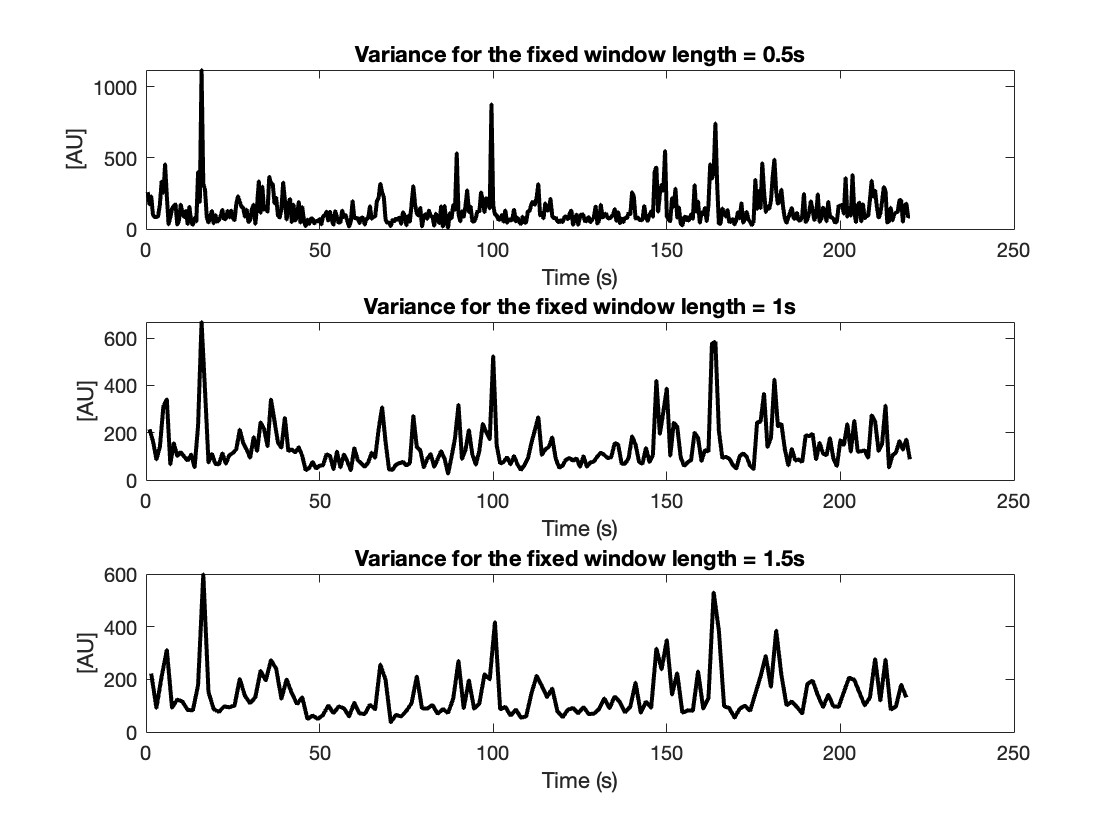
\includegraphics[width=\linewidth]{figure/figure_2.jpg}  
    \end{minipage}

    \begin{minipage}{0.5\textwidth}  
        \centering
        \textit{Comment:} 
        As the window duration increases, the magnitude of mean and variance decrease.
        The reason for the magnitude decrease is because longer time duration can include more data point
        which will average certain small duration with extrme high value(decrease mean) or some samll duration 
        with values change very fast(decrease variance.)
        
    \end{minipage}
    \hfill  
    \begin{minipage}{0.48\textwidth}  
        \centering  
        \begin{tabular}{|c|c|c|}  % Adjusted to 4 columns
        \hline
        Window Length(s)& Variability of Variance & Variability of Mean  \\
        \hline
        0.5 & 12615.04  & 10.93 \\
        1 & 9656.58  & 1.47  \\
        1.5 & 8073.51  & 1.16 \\
        \hline
        \end{tabular}
    \end{minipage}
    


    \subsection{Task B and C}
    %figure3
    \begin{minipage}{0.5\textwidth}  
    \centering
    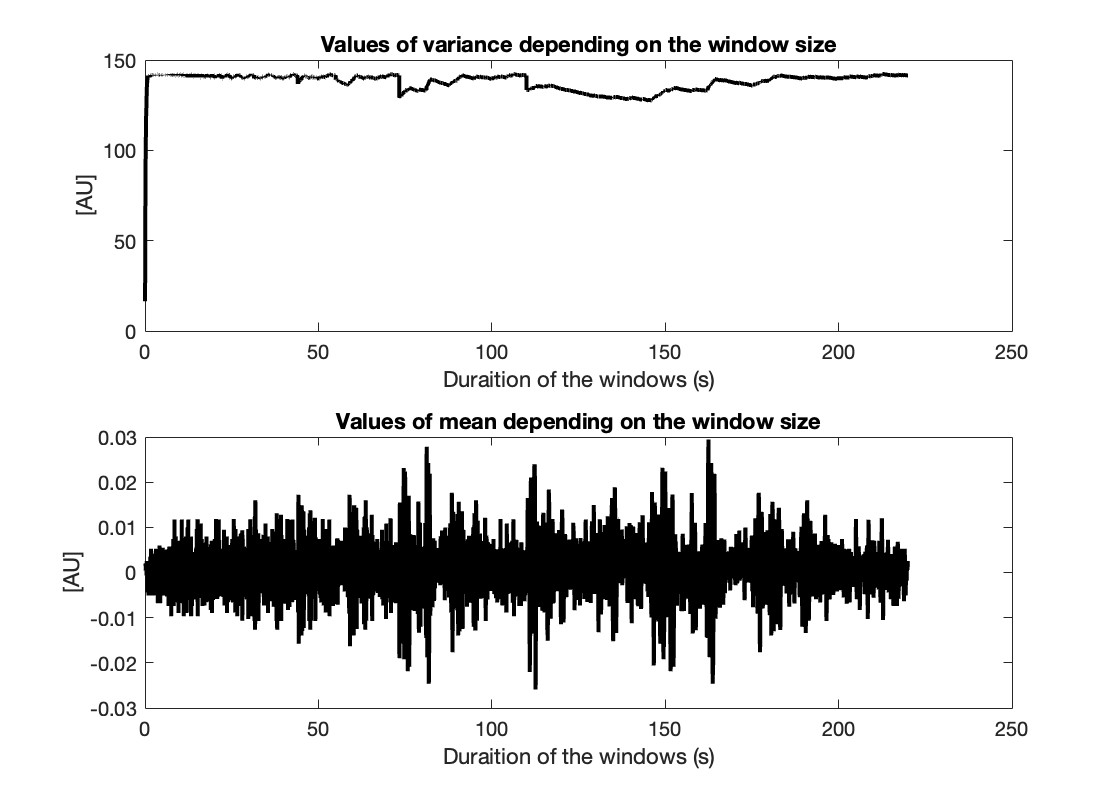
\includegraphics[width=\linewidth]{figure/figure3.jpg}  
    \end{minipage}
    \hfill  
    %figure4
    \begin{minipage}{0.48\textwidth}  
    \centering  
    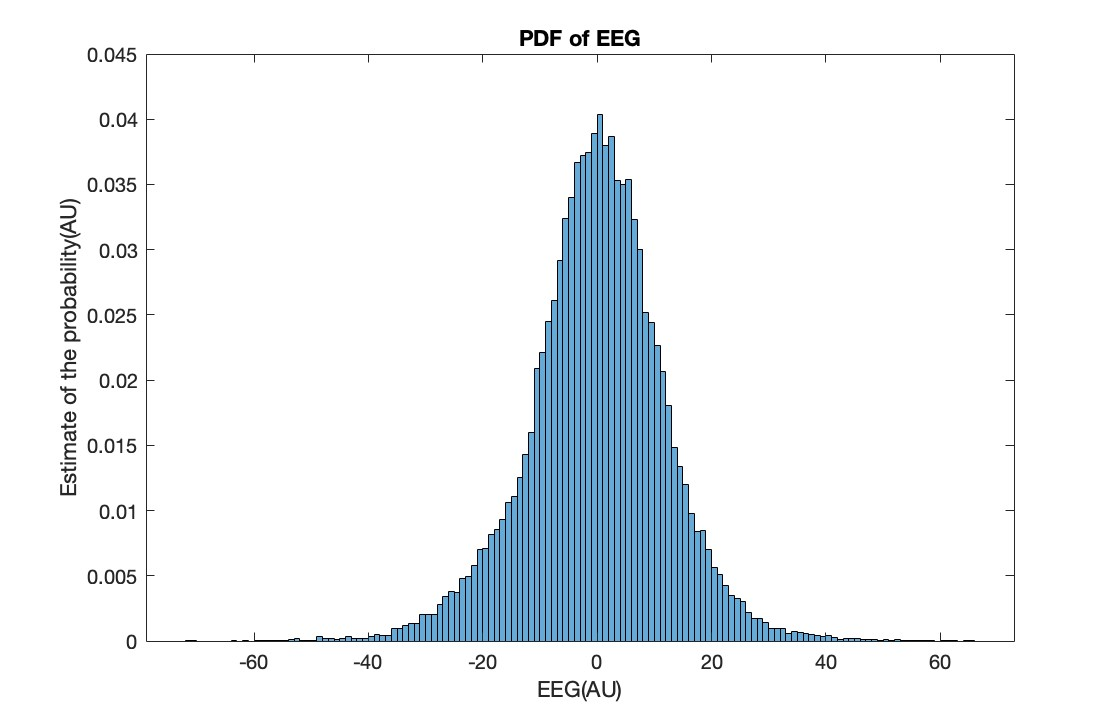
\includegraphics[width=\linewidth]{figure/figure4.jpg}  
    \end{minipage}
    The left figure above show the average values of variance and mean aganist the duration of window.
    The right figure above show the estimates of probability density function(PDF) for the EEG signal.
   
    
    \newpage
    
    
    
    \section{Laboratory 8}
    \begin{minipage}{0.5\textwidth}
        \subsection{Task A }

        The figure at the left side is the mean periodogram 
        applying the rectangular window with the window size at 0.2, 0.5
        and 2s. 

        \vspace{0.15cm}

        \subsection{Task B}

        \vspace{0.15cm}

        \centering
        %table2
        \begin{tabular}{|c|c|c|c|}  % Adjusted to 4 columns
            \hline
            Window Length(s)& 0.2 & 0.5 & 2  \\
            \hline
            Bias & 4.8186 & 2.0074 & 1.0311\\
            \hline
        \end{tabular}
        
        \vspace{0.3cm}

        The table above is the estimates' bias of the rectangular window with different 
        length.

        \vspace{0.15cm}
        \textit{Comment:} 
        The decrease in bias with an increase in window length can be explained by the fact that 
        applying a rectangular window in the time domain is equivalent to 
        convolving with a sinc function in the frequency domain, 
        where the PSD is calculated. 
        A wider time window results in a sinc function with a narrower main peak, 
        which ideally isolates a certain frequency and more accurately identifies its power. 
        Therefore, as the window length increases, the bias decreases.
    \end{minipage}
    \hfill
    %figure5
    \begin{minipage}{0.5\textwidth}
        \centering
        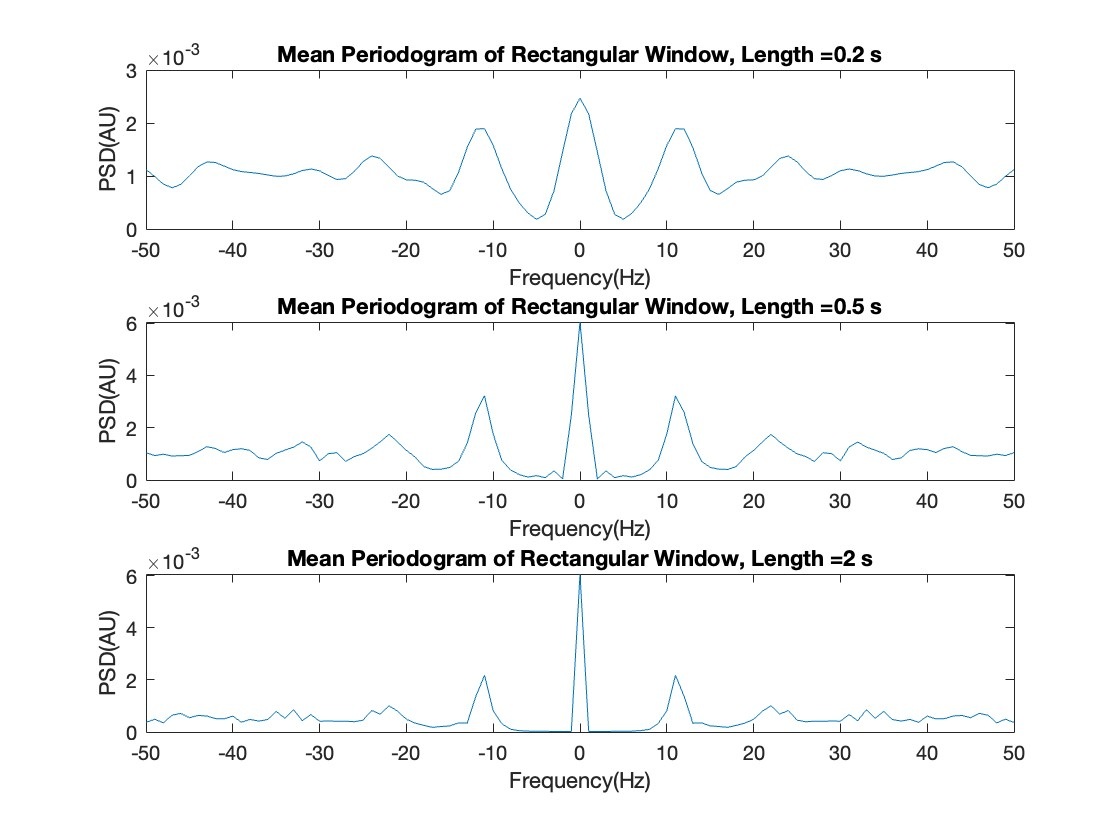
\includegraphics[width=\linewidth]{figure/figure5.jpg}
    \end{minipage}

    \subsection{Task C}
    %figure6
    \begin{minipage}{0.5\textwidth}
        \centering
        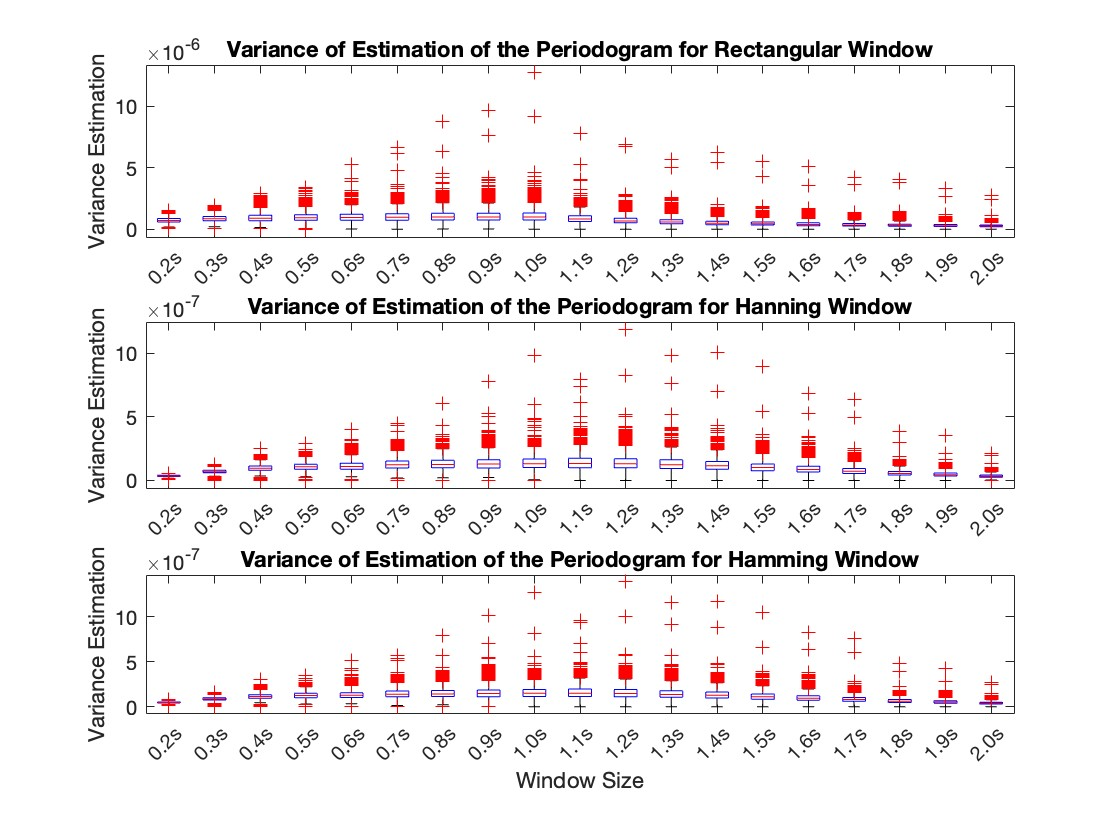
\includegraphics[width=\linewidth]{figure/figure6.jpg}
    \end{minipage}
    \begin{minipage}{0.48\textwidth}
    The figure at the left side is the the estimate of the variance of the 
    periodogram aganist the window length for 3 different types of window
    (Rectangular, Hanning and Hamming).

    \vspace{0.15cm}

    
    \end{minipage}

    \textit{Comment:}
    When the window length is between approximately 0.7 and 1.7 seconds, 
    the power at certain frequencies shows a high degree of variability across 35 observations. 
    This may be explained by the fact that different neural activity is captured within this range of window lengths, 
    resulting in a pronounced variability in power for these frequencies. 
    High variance for particular frequency on the PSD, 
    implying some observations have very high power that frequencies, while the others might have low power.
    This is expected, since there is a random variability of discharge around the average discharge time, which is stated in the question.
    With window lengths shorter than this range, 
    the signal might be divided in such a manner that each part contains less variability, 
    as the segmentation could miss capturing the more active periods of neural activity. 
    On the other hand, 
    when the window length is longer, 
    it includes more samples with less pronounced neural activity. 
    This additional data can dilute the variability, 
    leading to a more even distribution of power among the frequencies.

    Furthermore, the Hanning and Hamming windows display smaller variances compared to the rectangular window. 
    This reduction in variance is likely due to the decreased edge discontinuity associated with these windows, as opposed to the sharp discontinuities introduced by the rectangular window.
    \newpage



    \section{Laboratory 9}
    \subsection{Task A}
    \begin{minipage}{0.5\textwidth}
        \centering
        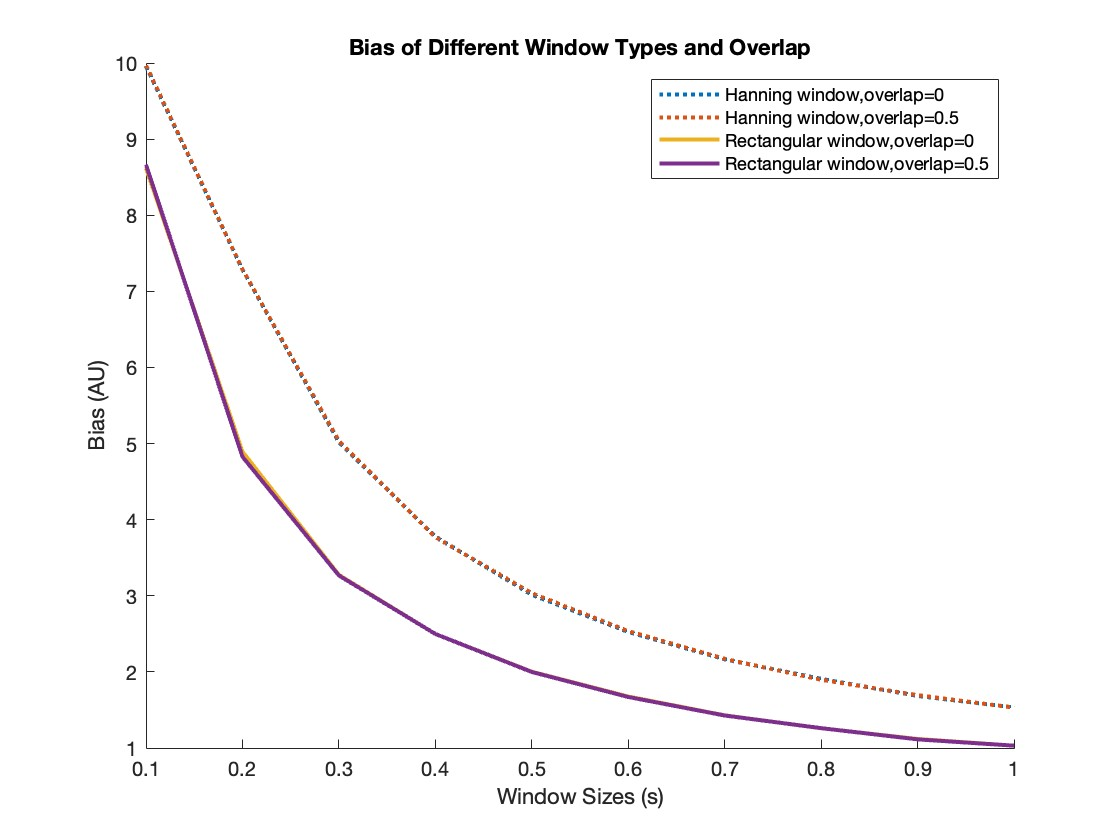
\includegraphics[width=\linewidth]{figure/figure7.jpg}
    \end{minipage}
    \hfill
    \begin{minipage}{0.5\textwidth}
        \centering
        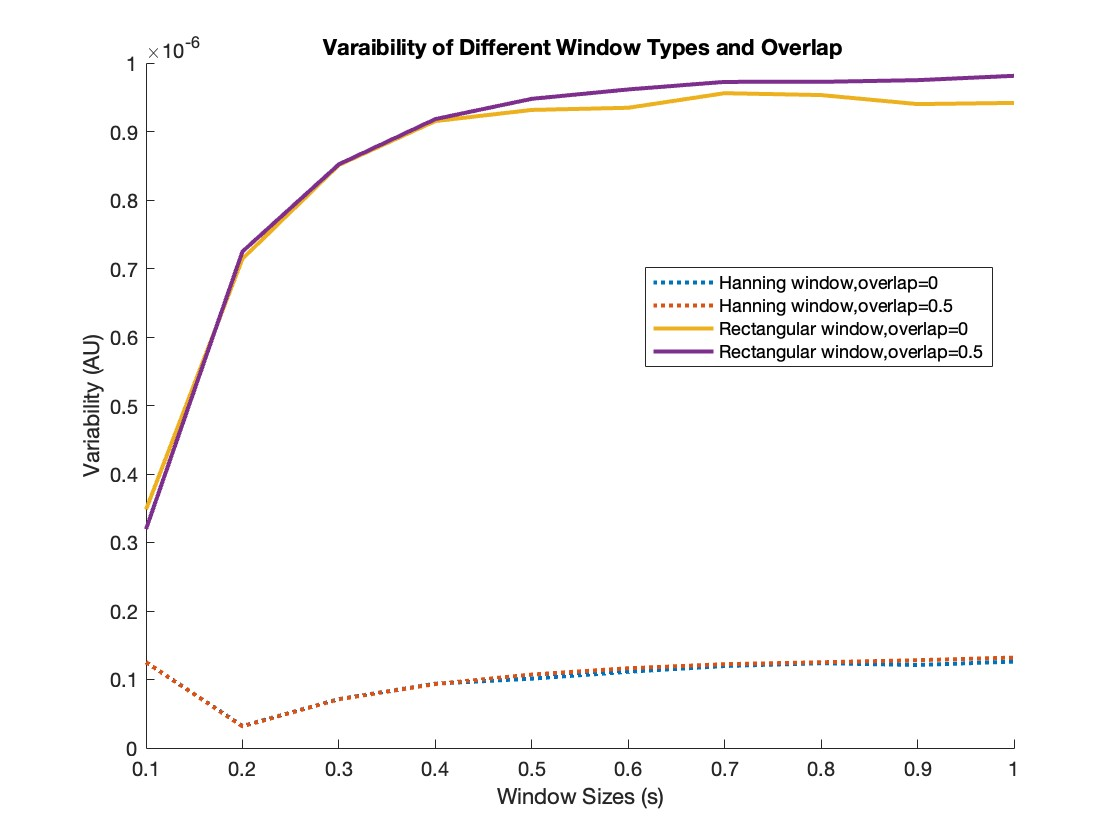
\includegraphics[width=\linewidth]{figure/figure8.jpg}
    \end{minipage}
    The two figure above illustrate the bias and variability of the PSD estimate 
    aganist the window length. Each plot shows the effect of different window type(rectangular and hanning) 
    with different overlap factor(0 and 0.5).

    \textit{Comment: }
    Overlap factors (0 and 0.5) do not significantly affect either bias or variability, 
    regardless of the window type or length. 
    As the figures illustrate, 
    lines representing different overlap factors show negligible differences 
    for both bias and variability when using rectangular and Hanning windows.

    Concerning bias (as depicted in the left figure), 
    it decreases as the time window widens. 
    This can be attributed to the fact that 
    employing a window (both hanning and rectangular) in the time domain 
    corresponds to a sinc function (for hanning, it's something looks like sinc with less other peaks) convolution in the frequency domain. 
    The broader the window, 
    the more narrow the main peak of the sinc function becomes, 
    which in turn reduces bias. 
    Moreover, 
    the Hanning window tends to exhibit greater bias compared to the rectangular window. 
    This might be due to the sharper discontinuities at the edges of the rectangular window 
    as opposed to the smoother edges of the Hanning window.

    Regarding variability(right figure), 
    it generally increases with longer window lengths. 
    A shorter window permits the generation of more window samples, 
    and a larger number of samples can reduce variance. 
    The rectangular window demonstrates higher variability compared to the Hanning window; 
    this is likely due to the reduced spectral leakage in the Hanning window, 
    which implies that less power from other frequencies is included when calculating the power of a specific frequency. 
    The leakage effect is more pronounced for the rectangular window 
    because it has multiple peaks aside 
    from the main lobe, 
    capturing power from frequencies unrelated to the one being measured, 
    which results in increased variability.

    \subsection{Task B}
    \subsubsection{Window Length Change}
    When the window length is increased, 
    bias tends to decrease due to a narrower sinc function main peak in frequency domain analysis, 
    while variability increases because of the reduced number of windowed segments.

    \subsubsection{Overlap Factor Change}
    Variations in the overlap factor, 
    at 0.5, 
    have negligible effects on bias and variability. 
    This suggests that the expected increase in sample count from overlapping does not significantly reduce variability.

    \subsubsection{Window Type Change}
    Comparatively, 
    the Hanning window results in 
    lower variance 
    and higher bias than the rectangular window. 
    The wider main peak and reduced side peaks of the Hanning window's frequency response, 
    explain its lower variance and higher bias.
    \end{document}

